\subsubsection{Motivation for Directional Detection}

There are three predicted nuclear recoil signatures of particle dark matter1: 1) an excess in the observed nuclear recoil rate over the predicted background from radioactive impurities and neutrino scattering; 2) an annual modulation in the nuclear recoil rate and energy spectrum due to the motion of the earth around the sun; and 3) a fixed dipole-shaped angular recoil distribution in galactic coordinates, resulting from the motion of the galactic disk with respect to the dark matter halo -- in a terrestrial detector, this last effect is seen as a DM wind, with a direction that oscillates due to the large tilt angle between the earth's spin axis and the luminous plane of the Milky Way (and solar motion).  A direct detection experiment can pursue one or several of these signatures.

Most leading direct detection experiments to date, such as the liquid noble gas detectors described above, have primarily aimed to detect Signature 1.  Signature 2 was used by DAMA/LIBRA~\cite{Bernabei:2019ajy} to claim a detection of dark matter that has not been confirmed by subsequent experiments.  This second signature can be used even in the presence of backgrounds, but requires exquisite detector stability and a large number (1000s) of observed DM events to detect the relatively small (few-percent-level) modulation magnitude, and is subject to interference from temperature effects and cosmic ray-induced background, which also are expected to have an annual modulation.  Signature 3 requires significantly more complex detectors, capable of reconstructing the directions of low-energy nuclear recoils, not strictly required for Signatures 1 and 2.  On the other hand, because the majority of recoils are expected to point to a single hemisphere in galactic coordinates, the effect is large, so that only a few detected DM events are required.  Neither radio-impurities nor solar neutrinos can mimic the dipole signature expected from dark matter~\cite{OHare:2015utx}.  Its magnitude and experimental robustness makes the directional dipole signature a ``smoking gun" signature of DM.

\begin{figure}[ht!]
\begin{center}
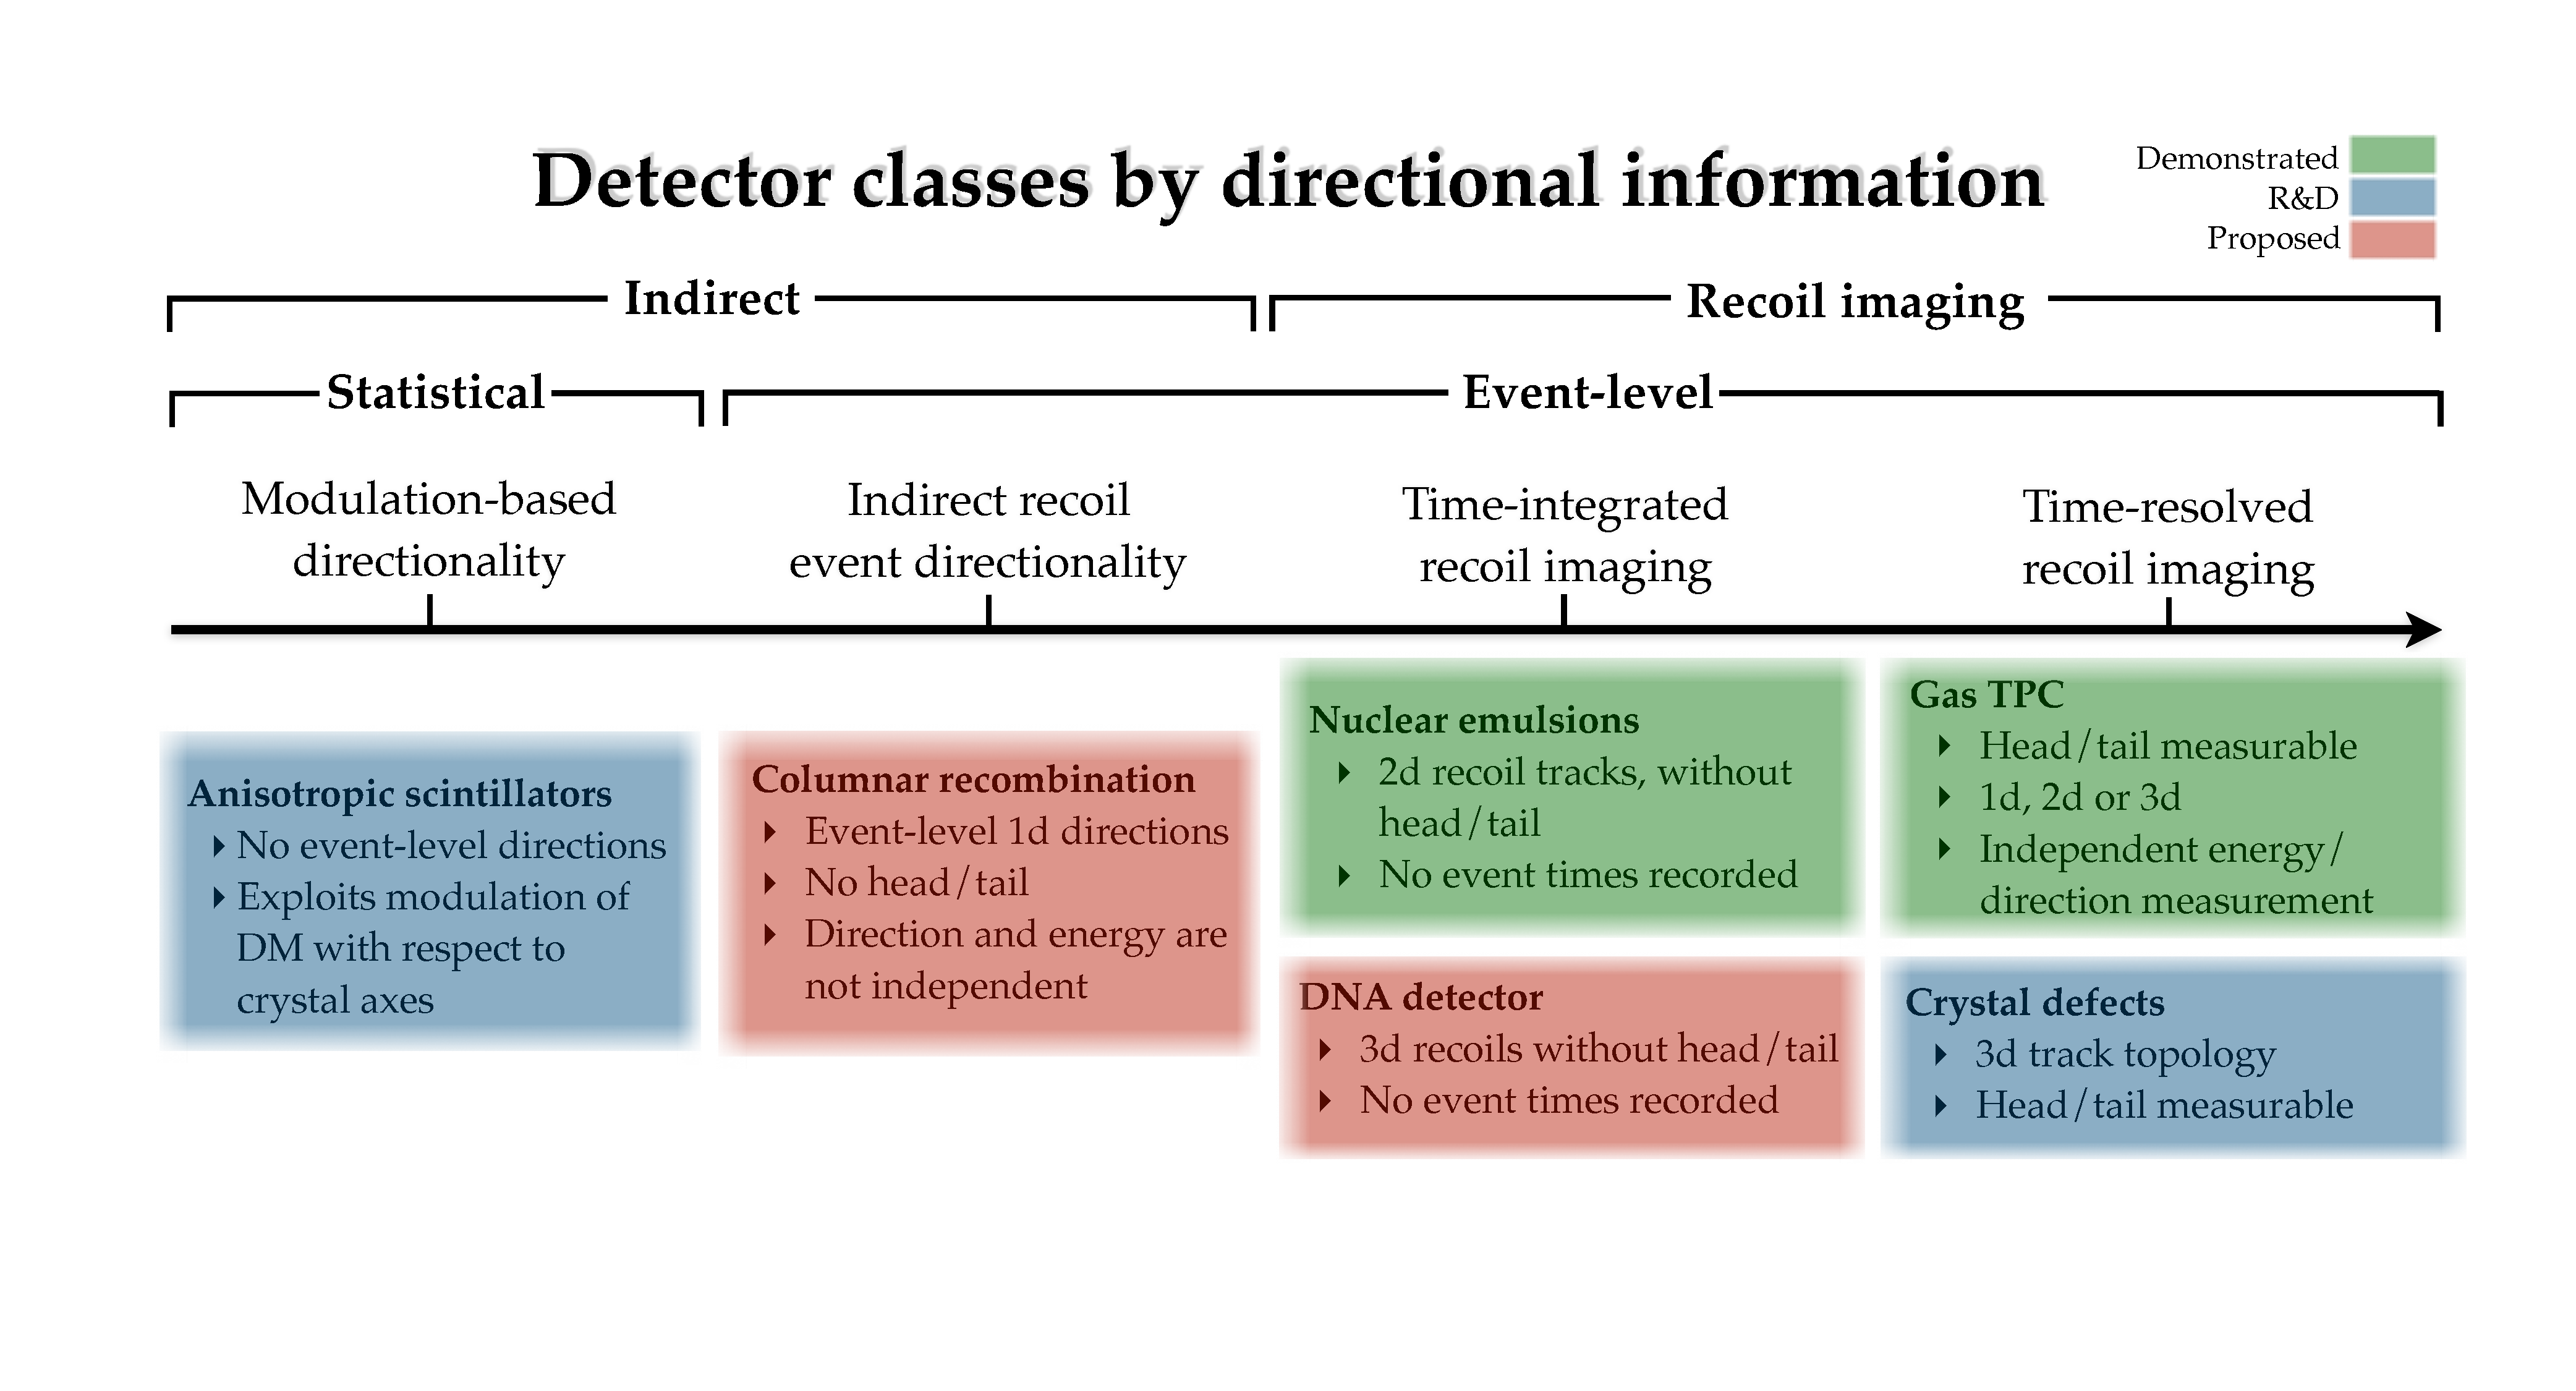
\includegraphics[width=0.9\columnwidth]{figures/DetectorClassTableAR.pdf}
\caption{Various classes of directional detector ordered roughly (from left to right) from least to most directional information that they are able to access. The minimal amount of directionality is for an experiment that can only infer some kind of direction-dependence from a statistical distribution of event information. On the other hand, a fully direction-sensitive experiment is one that can access up to 3D information on each recoil track individually, and in real-time. This is possessed only by gas TPCs and crystal defect approaches. Figure adapted from Ref.~\cite{Vahsen:2021gnb}}\label{directional_classification}
\end{center}
\end{figure}

The various strategies for directional recoil detection are reviewed in Ref.~\cite{Vahsen:2021gnb}, and summarized in Fig.~\ref{directional_classification}.  Directional detection can be achieved either directly by imaging the nuclear recoil trajectory, or indirectly by inferring the direction from a proxy variable.  We will see below that low-density gas TPCs are capable of direct recoil imaging. Indirect approaches include anisotropic light yield in crystals, and anisotropic ionization detection due to columnar recombination in liquid or gas, which have not yet been demonstrated at the energies relevant for DM searches.

With a recoil-imaging detector, it is possible to observe the directional galactic dipole signature with as few as 5--10 detected DM events if the performance is at the level of the following or better~\cite{Vahsen:2021gnb}: recoil axis angular resolution $\leq 30^\circ$; efficiency for correctly detecting the recoil head/tail $>$ 80\%; offline rejection of electron-recoil background by factors $>10^5$.

The NEWS collaboration (based in Japan and Italy) is pursuing directional recoil detection in emulsions~\cite{NEWS:2016fyf} and making good progress.  Outside the particle physics community, quantum defects in wide-bandgap semiconductors have also been proposed to achieve directional sensitivity at solid-state densities \cite{Rajendran:2017ynw,Marshall:2020azl,Ebadi:2022}.  The incident particle's direction would be stored as a durable, submicron track of crystal lattice damage, which could be mapped using solid-state quantum sensing methods. Early R\&D has focused on nitrogen-vacancy defects in diamond \cite{Marshall:2020azl,Marshall:2021kjk,Marshall:2021xiu} to establish the feasibility of directional readout of such tracks. 
The remaining world-wide groups working on recoil imaging are pursuing low-density gas TPCs, where keV-scale nuclear recoils can be mm in length, while charge diffusion is of order 100~$\upmu$m, which allows for the directional reconstruction of nuclear recoils.

Recently, most groups worldwide that are pursuing directional detection in gas TPCs joined forces to form the CYGNUS Detector R\&D collaboration.  The CYGNUS collaboration proposes to build a $\ge 1000~{\rm m}^3$ recoil-imaging gas target TPC.  The proposed detector consists of a large number of smaller modules, which allows for the large volume to be distributed across multiple underground laboratories. Gas detectors have lower target mass per unit volume than liquid or solid target detectors, but can detect even individual electrons of ionization with $\mathcal{O}(100~\upmu$m) spatial resolution.  As we are rapidly approaching the neutrino fog, DM detectors are guaranteed to see an irreducible background soon. This is a background which can be clearly separated from DM signals via directionality. The neutrino scattering events expected in the neutrino fog can also be exploited as a signal.

The approximate timeline for CYGNUS worldwide is: 1) 2022-2025: 1~m$^3$ detectors to be constructed and start operation in the UK, Japan, Italy, US, and Australia; 2) 2025-2035: 10~m$^3$ detectors: CYGNUS HD10 module (electronic readout) to be jointly constructed and operated in the US; a CYGNO detector (optical readout) program is planned and funded in Italy; detectors in Japan, the UK, and Australia are also planned; and 3) 2024-2042+: 1000~m$^3$ detectors, with construction of the facility to begin in 2030.

The largest directional DM detector prototypes to date have been 1~m$^3$ in volume, and were built by the DRIFT~\cite{Battat:2016xxe} and DMTPC~\cite{Ahlen:2010ub} collaborations. Both detectors were designed to search for 100-GeV DM particles, and have limited directionality for recoil energies below 50~keVr.  Recently, smaller R\&D detectors in the US have shown that the particle identification and event-level recoil directionality required for a directional discovery with only 5-10 events can be achieved even at sub-10-keV energies. Modern MPGD-based detectors utilizing electronic readout~\cite{Jaegle:2019jpx} with charge multiplication gains exceeding 3000--9000, result in ionization threshold of order 30~eV, and detection of sub-10-keV recoils. CYGNUS HD recently achieved both the desired low-energy particle identification and directional capabilities with 3D convolutional neural networks (3D CNNs). The desired end result would be a CYGNUS detector operating at the fundamental performance limit where individual primary electrons are counted in 3D at $100~\upmu$m$^3$ spatial resolution, with diffusion kept minimal even at large drift lengths through negative ion drift. Recent R\&D with GridPix charge readout ~\cite{Ligtenberg:2021viw} has demonstrated the feasibility of this on a smaller scale. The CYGNUS-HD members in the US are currently building prototypes to demonstrate sub-10-keV directionality at the 40~L and then 1000~L module scale.  For further detail, we refer the reader to Refs.~\cite{Vahsen:2021gnb,Vahsen:2020pzb,SnowmassIF53}.